\documentclass[10pt]{article}
\usepackage[letterpaper,margin=0.55in]{geometry}
\usepackage{graphicx,xcolor,enumitem,multicol}
\usepackage[hidelinks]{hyperref}
\definecolor{navy}{HTML}{1B2F4B}\definecolor{sea}{HTML}{2E7DB5}
\setlist{nosep,leftmargin=1.1em}
\pagestyle{empty}
\setlength{\parindent}{0pt}
\newcommand{\head}[1]{\vspace{5pt}{\color{navy}\large\bfseries #1}\par\vspace{2pt}}
\begin{document}
{\color{navy}\LARGE\bfseries A 1\,m RC Foiling Beach Catamaran: Design, Analysis and Build Plan}\par
\vspace{2pt}{\large Filip Maleev \quad|\quad Colorado College, Mathematics \quad|\quad September 2026}\par
\vspace{6pt}
\begin{minipage}[t]{0.49\textwidth}\vspace{0pt}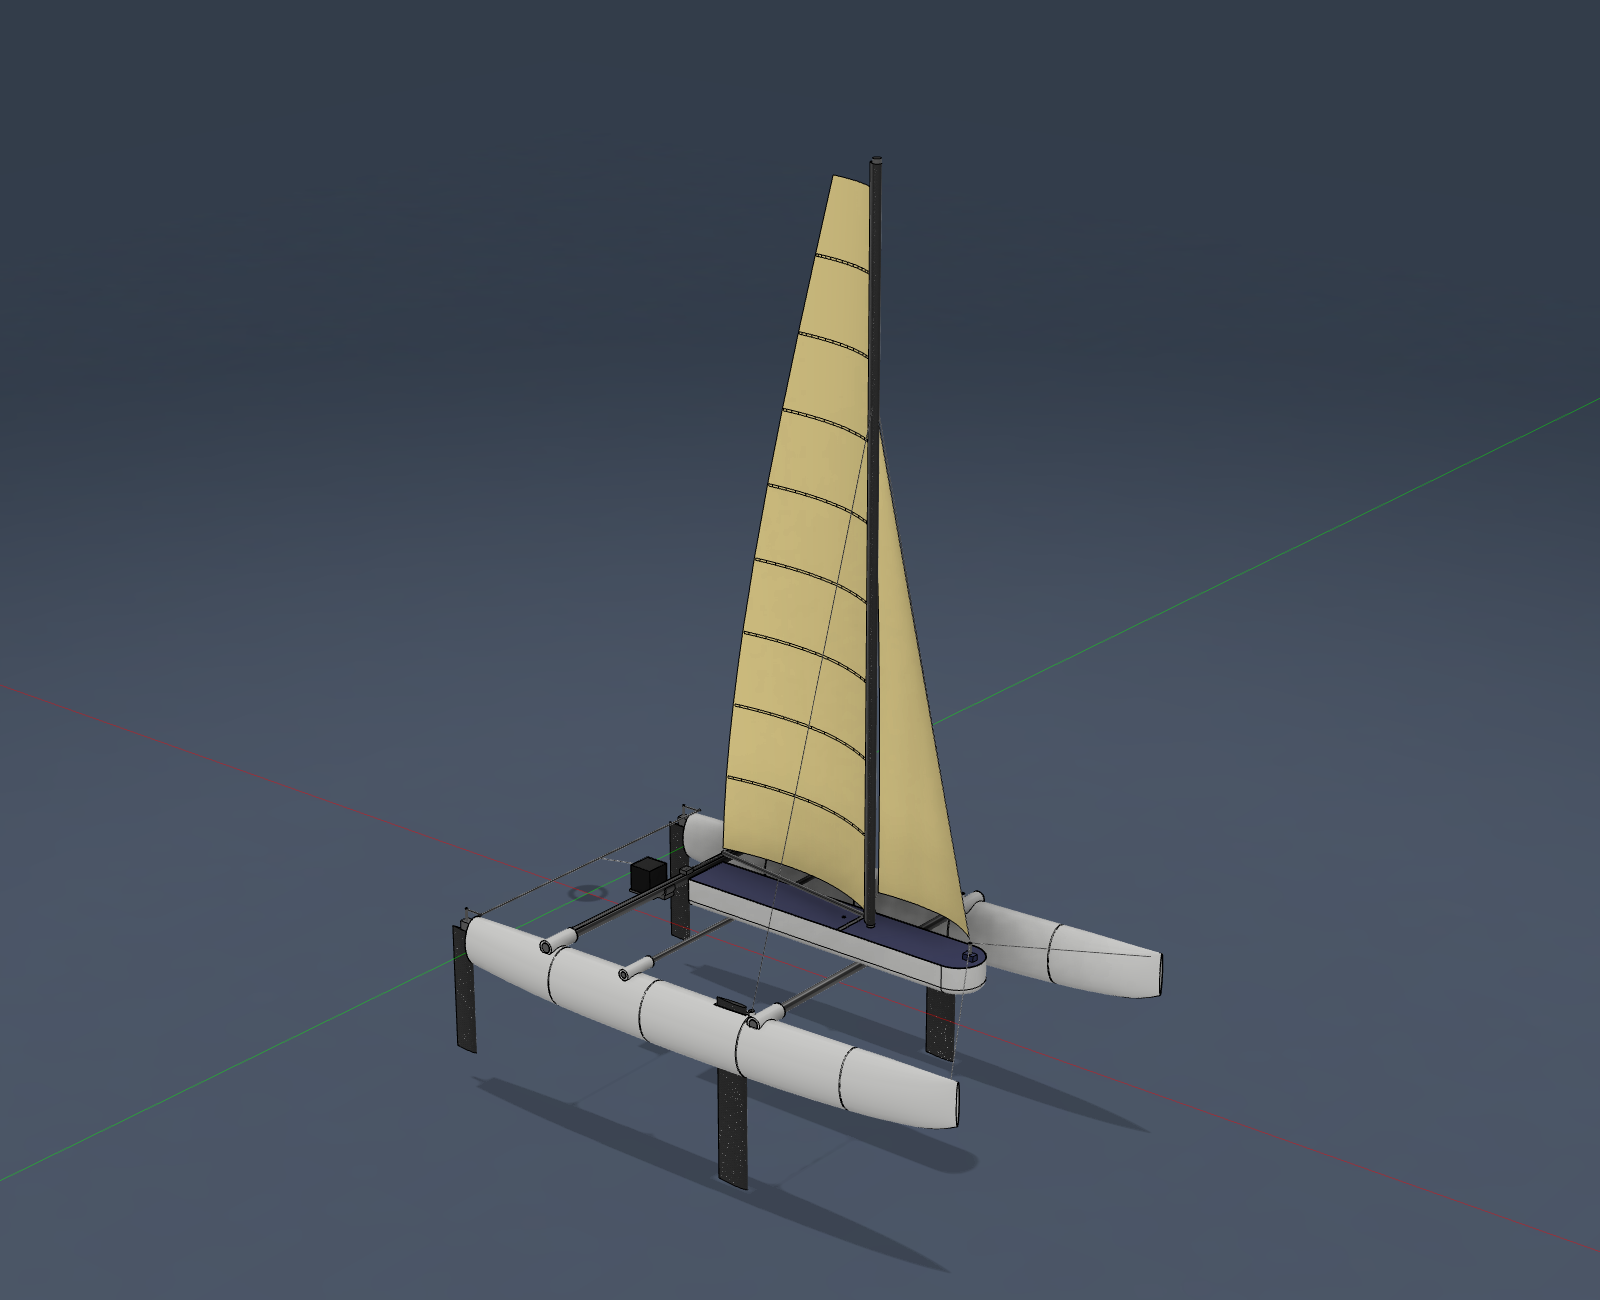
\includegraphics[width=\linewidth]{../images/build_first_v1.4.png}\end{minipage}\hfill
\begin{minipage}[t]{0.49\textwidth}\vspace{0pt}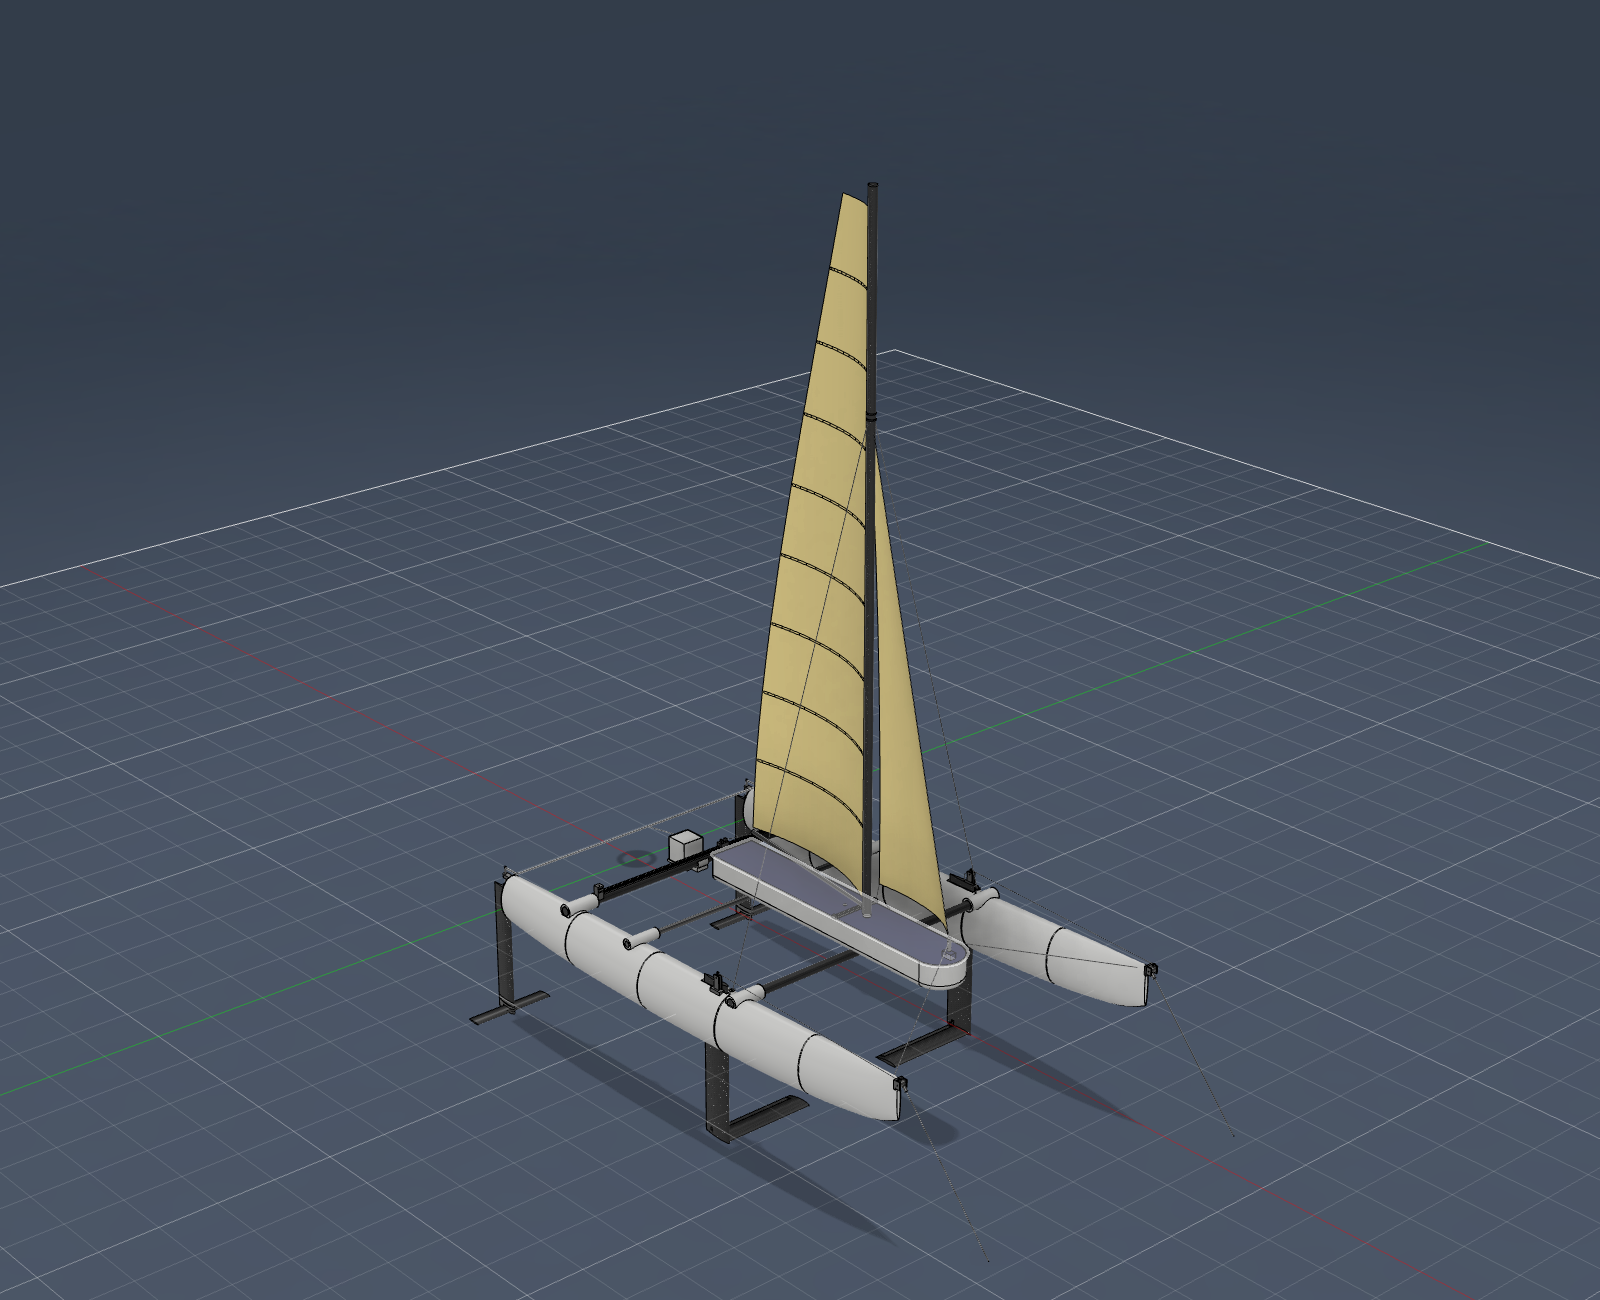
\includegraphics[width=\linewidth]{../images/foiling_v2.3.png}\end{minipage}\par
{\small Build-first version (daggerboards) and foiling version (v2.3 L-foils, wand-driven flaps), Autodesk Fusion.}
\begin{multicols}{2}
\head{Goal}
A radio-controlled catamaran that follows full-size beach cats (Hobie~16, Nacra~17), can be 3D-printed and built from off-the-shelf RC parts, can fly on hydrofoils, and whose behaviour is predicted before it is built.

\head{What was done}
\begin{itemize}
\item \textbf{Parametric CAD} in Autodesk Fusion, driven through its API: 1\,m hulls printed as sealed PETG segments, a beach-cat rig trimmed by three sliders, two appendage options, a 0.6\,m first build, clearance sweeps, and mass and inertia exported for analysis.
\item \textbf{Velocity prediction}: ITTC-57 friction, Michell thin-ship wave resistance with catamaran interference (checked on the Wigley hull), foil and appendage drag, and sails eased for heel and bow-down limits.
\item \textbf{Foils}: lifting-line wings with wand-driven flaps; flying trim in heave and pitch, roll authority, coupled heave--pitch stability, and a time-domain take-off simulation.
\item \textbf{Flight simulator} (web page, same physics) and a search of 306,180 foil designs under limits on stress, deflection, Reynolds number, pitch stability and damping, with depth margins and robustness checks.
\item \textbf{Build plan}: every fitting drawn and printable (tracks and cars, gudgeons, wing-mast fairing, gooseneck, ride-height linkage); costed parts lists (every price read from a retailer page), build manuals for the 0.6\,m and 1\,m boats, and a tow-test plan for the foils.
\end{itemize}

\head{Findings}
\begin{itemize}
\item Fixed-incidence foils have no heave stability; a wand-driven flap on each foil makes heave and pitch stable (least damping ratio 0.69).
\item The first optimized foils (v2.1) would not have flown: at speed the sail drive's bow-down couple makes the elevators push down, and at $+4^\circ$ they pitch the boat nose-down until they leave the water. The adopted v2.3 foils set the elevators at $-0.5^\circ$ and fly level.
\item Near take-off the foils have no roll authority left, so flying at 60$^\circ$ needs 8.9\,kn against 7.1\,kn on a beam reach; taking off on a reach and heading up keeps it flying at 60$^\circ$ from 8.2\,kn.
\item Predicted speed on a beam reach: build-first 2.65\,m/s in 8\,kn; foiling 4.53\,m/s in 12\,kn.
\end{itemize}

\head{Deliverables}
Technical paper, A0 poster, build manual with 1:1 sail patterns, tow-test plan, interactive simulator, STEP/Fusion models and print-ready STLs. Checks in the code: 28 of 28 foil rules and 30 of 30 design rules pass.

\head{Cost}
0.6\,m first build \$257.37; 1\,m build-first boat \$384.49; foiling kit \$101.17 (September 2026 retailer prices, before shipping and tax).

\head{Next}
Build and GPS-log the 0.6\,m boat and compare with its predicted 2.1\,m/s in 8\,kn; build the 1\,m boat; tow-test the foils against the plan's predictions, then fly.
\end{multicols}
\vfill
{\footnotesize\color{black!65} All performance figures are model predictions; nothing has been tested on the water yet. Developed with Claude (Anthropic) as an AI engineering assistant for the CAD scripting, analysis code and documents.}
\end{document}
